%-----------------------------------------------------------------
\begin{plSection}{Typesetting this document}

This document was typeset using Mik\TeX{} $21.3$ 
\cite{Schenk:2017:Miktex} 
and {\TeX}works $0.6.5$ \cite{KewLoffler:2017:Texworks} 
on \textsc{Windows} $10$. 
I used \texttt{arara} \cite{CeredaEtAl:2021:Arara} 
to run \texttt{xelatex}, \texttt{biber}, \texttt{makeglossaries},  
and
\texttt{texindy: { markup: xelatex }}.
I believe only Mik\TeX\  and {\TeX}works are Windows specific; 
the actual typesetting tools should be usable on Linux and MacOS 
as well.

See also \cite{Talbot:2012:LatexNovices,Talbot:2013:LatexPhD}.

\begin{plScreen}
{Configuring {\TeX}works for \texttt{arara}.}
{fig:arara}
\centering
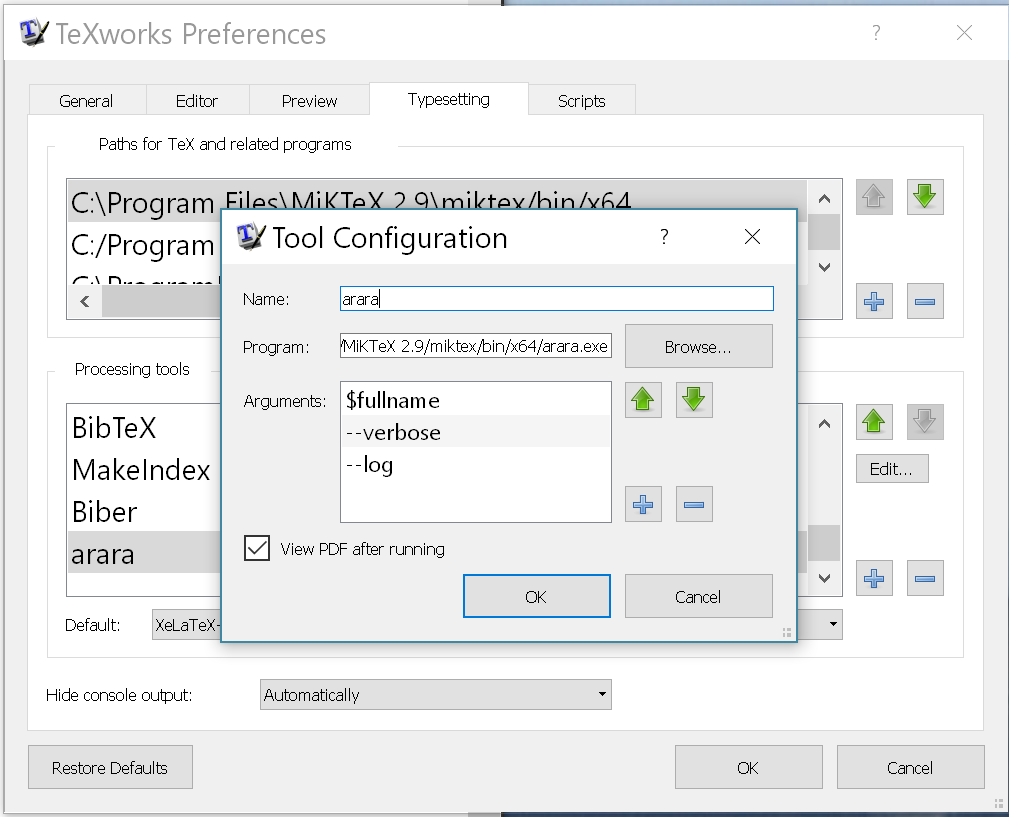
\includegraphics[scale=0.75]{arara.png}
\end{plScreen}

As of 2021-03-16, I am defaulting to 'upright' math text.
I am considering trying sans symbols (sum, integral) 
as the default as well,
but I'm not sure if the existing sans math fonts are as well
developed as the others, especially for non-letter symbols.

Goals are:
\begin{enumerate}
\item Readability (at least subjectively). Prefer top-down over
    bottom-up understanding. In particular, it should be easy to
    pick out the general structure of an expression, ignoring
    less important details.

\item General appearance should be something like regularized,
    cleaned up, good handwriting. To me this suggests upright
    sans letters and compatible symbols.

\item Math expressions should be visually distinct from regular
    text, especially when mixed together --- but not so much
    that it disturbs the flow of reading. To me, this suggests
    serif fonts for text and, again, sans for math, upright
    for both, and restraint in weight variation.
\end{enumerate}

I am aware of ISO 80000-2:2019, but haven't read it,
since the price is about US\$170 and I doubt I would agree with
their choices. Indirect sources suggest that in ISO 80000-2
most symbols are set in italic, which I find difficult to read,
and believe should be restricted, if used at all, to placing
emphasis on very short pieces of text, on the order of a word
or short phrase.~\cite{wiki:TypoConventionsMath}
And even in that case, and contrary to most
advice I've seen, I prefer slanted faces to italic
(one agreeing opinion, for text at least: 
\citeAuthorYearTitle{RoddTornqkvist:2009:LMSStyleGuide}.
My subjective feeling is that italic text,
in most fonts, is read more-or-less single letter at a time,
rather than word or phrase at a time. I think the same applies
to mathematical expressions, forcing the reader work bottom up,
to first parse out individual letters/symbols and then
consciously re-assemble them, rather than grasping
the expression as a whole, and then acquiring details top-down.


\vfill

\end{plSection}%{Typesetting}
